\documentclass[a4paper,10pt]{article}
\usepackage[left=2cm,top=3cm,right=3cm,bottom=3cm]{geometry}
\usepackage{enumerate}
\usepackage{multicol}
\usepackage{verbatim}
\usepackage{float}
\usepackage{amssymb,amsmath} 
\usepackage{amsthm}
\usepackage[pdftex]{graphicx}
\usepackage{rotating}

%\usepackage{bookmarks=true}{hyperref}
\usepackage{listings}
\usepackage[pdftitle={Netfilter/iptables},pdfpagemode=UseOutlines,
colorlinks=false,pdfauthor={Andrew Rimes and Kreshnik Mati},
bookmarks=true,pdftex=true,linkbordercolor={1 1 1}]{hyperref} 
\pdfpagewidth=21.6cm
\pdfpageheight=27.9cm
\usepackage{times} %use PS fonts for PDF
\usepackage{courier}
\usepackage{helvet}
\usepackage{cmap} % searchable PDF

\newcommand{\code}[1]{\texttt{{#1}}}
\newcommand{\figref}[1]{[fig. \ref{#1}]}
\newcommand{\cref}[1]{[\ref{#1}]}
%\bibliographystyle{prsty} % Choose Phys. Rev. stylle for bibliography
\bibliographystyle{plain}


\lstset{language=C,basicstyle=\footnotesize,frame=single,showstringspaces=false,breaklines=true,breakatwhitespace=true}
\begin{document}
\title{\textbf{Project}:\\Netfilter/iptables}
\author{Andrew Rimes - cs253030\\Kreshnik Mati - cse93062\\CSE4221 - F09}
\date{December 8, 2009}

\maketitle
\thispagestyle{empty} 

\newpage

\setcounter{tocdepth}{3}
\tableofcontents


\newpage
\raggedright

\section{Overview}

\verb|iptables| usually refers to the framework and associated modules that make up the firewall and NAT subsystem in the Linux kernel. (It is more probably called \verb|X_tables| since it supports several network protocols including IPv4, IPv6 and ARP.) \verb|iptables| is also the name of the userland program used for manipulating the in-kernel data structures that define the firewall and NAT rules. The framework provides hooks for general \textit{packet mangling} and can be used to implement kernel modules that in someway intercept, modify or track packets flowing through the Linux TCP/IP stack, e.g. an IPSec VPN could be implemented in this manner. This report will cover some of the major data structures that make up the firewalls rules and matching mechanism (\ref{rule-tables}), the connection tracking system (\ref{conntrack}) and the registration system(\ref{registration}) that allows modules to be registered to event hooks.


\section{Rule Tables}\label{rule-tables}

\subsection{Overview}

An IP table is made of multiple chains; a chain is a list of rules
associated with one or more hooks. Each rule consists of one or more
matches, terminated by a target. The target is the action performed
when a rule is entirely matched. The data structures are designed
such that they can be used in both kernel mode and user mode by
the \verb|iptables| command.

\subsection{Data Structures}

\subsubsection{ip\_tables.h/ipt\_ip}\label{ipt_ip}

This struct specifies the minimal IP header information needed
to to identify a packet. The \code{src} and \code{dst} fields identify
the source and destination IP addresses, and \code{smsk} and
\code{dmsk} identify the source and destination masks so that ranges
of IP addresses can be specified in the rule, e.g. 192.168.0.0/24
would match all IPs in the 192.168.0.0 subnet\cite{tcpip-illustrated}. The \code{initface} and
\code{outiface} fields specify inbound and outbound interfaces, and
\code{iniface\_mask} and \code{outiface\_mask} allow the user to specify several
interfaces at once. The protocol number is stored in \code{proto},
e.g. it would be set to 6 for TCP. The fields \code{flags} and
\code{invflags} specified the IP header flags selected and not selected.

\begin{lstlisting}

struct ipt_ip {
	/* Source and destination IP addr */
	struct in_addr src, dst;
        /* Mask for src and dest IP addr */
        struct in_addr smsk, dmsk;
        char iniface[IFNAMSIZ], outiface[IFNAMSIZ];
        unsigned char iniface_mask[IFNAMSIZ], outiface_mask[IFNAMSIZ];

        /* Protocol, 0 = ANY */
        u_int16_t proto;

        /* Flags word */
        u_int8_t flags;
        /* Inverse flags */
        u_int8_t invflags;
};

\end{lstlisting}

\subsubsection{ip\_tables.h/ipt\_entry}

This structure defines the starting point of each of the firewall
rules, which are contained in arrays, i.e. tables.  The
\code{nf\_cache} bitfield shows what parts of the packet this rule
exams. The \code{target\_offset} field indicates the offset between
the beginning of the current rule (contained in the structure) and
where the \code{ipt\_entry\_target} begins. As indicated in the
comments, the target offset is equal to the size of the
\code{ipt\_entry} and the total number of matches. The
\code{next\_offset} is the sum of the entry, matches, and target,
which determines the position of the next rule's
\code{ipt\_entry}. The target, described elsewhere, is executed when
the rule matches. The \code{comefrom} field is a back pointer used by
the kernel to track packet traversal. Obviously, \code{counters}
stores packet and byte counts for the rule, i.e. how many have passed
through. The final, variable length field \code{elems} is where matches,
terminated by the target, are stored.

\begin{lstlisting}
struct ipt_entry
{
        struct ipt_ip ip;

        /* Mark with fields that we care about. */
        unsigned int nfcache;

        /* Size of ipt_entry + matches */
        u_int16_t target_offset;
        /* Size of ipt_entry + matches + target */
        u_int16_t next_offset;

        /* Back pointer */
        unsigned int comefrom;

        /* Packet and byte counters. */
        struct xt_counters counters;

        /* The matches (if any), then the target. */
        unsigned char elems[0];
};
\end{lstlisting}

\subsubsection{x\_tables.h/xt\_entry\_match (ipt\_entry\_match)}

This provides a thin layer of abstraction so that code can be reused
regardless of whether it is executing in the kernel or in user
space. We will discuss \code{xt\_match} since we are concerned with
the kernel\footnote{In some cases, structs have two names: one beginning with xt and one
without. This is a result of the unification of common code in
\code{ip\_tables}, \code{ip6\_tables} and \code{arp\_tables} into \code{x\_tables} (hence xt) -- a table
structure that can handle all three protocols.}.

\begin{lstlisting}
struct xt_entry_match
{
        union {
                struct {
                        __u16 match_size;

			/* Used by userspace */
                        char name[XT_FUNCTION_MAXNAMELEN-1];

                        __u8 revision;
                } user;
		struct {
                        __u16 match_size;

                        /* Used inside the kernel */
                        struct xt_match *match;
                } kernel;

                /* Total length */
                __u16 match_size;
        } u;

        unsigned char data[0];
};
\end{lstlisting}

\subsubsection{x\_tables.h/xt\_match}\label{xt_match}
This structure represents a match entry in a rule (possibly one of
many). It is fairly abstract and meant to represent all types of
matches.

The \code{list} is the standard doubly linked list used in
the Linux kernel; this simple struct has two fields, \code{prev} and
\code{nest}, and  is defined in \code{include/linux/list.h}. In this
case it is used to link together consecutive matches in the rule.
The \code{name} field stores the name of the current
table. The \code{revision} field stores the
current revision number of the data structure so that if it changes in
the future, backwards compatibility can be maintained.

The \code{match} field is a pointer to the Boolean function that
determines whether or not the packet will be matched. The \code{skb}
parameter is a pointer to a copy of the packet and
\code{xt\_match\_param} is a pointer to additional parameters the
match function can use to make the decision.

The function pointed to by \code{checkentry} is called when the user
attempts to add this type of match to the rule (whatever that type is). The struct
\code{xt\_mtchk\_param} (\ref{xt_mtchk_param}) is passed to make that decision. 

\begin{lstlisting}
struct xt_match
{
        struct list_head list;

        const char name[XT_FUNCTION_MAXNAMELEN-1];
        u_int8_t revision;

        /* Return true or false: return FALSE and set *hotdrop = 1 to                                                                                       
           force immediate packet drop. */
       bool (*match)(const struct sk_buff *skb,
                      const struct xt_match_param *);

        /* Called when user tries to insert an entry of this type. */
        bool (*checkentry)(const struct xt_mtchk_param *);

        /* Called when entry of this type deleted. */
        void (*destroy)(const struct xt_mtdtor_param *);

        /* Called when userspace align differs from kernel space one */
        void (*compat_from_user)(void *dst, void *src);
        int (*compat_to_user)(void __user *dst, void *src);

        /* Set this to THIS_MODULE if you are a module, otherwise NULL */
        struct module *me;

        /* Free to use by each match */
        unsigned long data;

        const char *table;
        unsigned int matchsize;
        unsigned int compatsize;
        unsigned int hooks;
        unsigned short proto;

        unsigned short family;
};
        
\end{lstlisting}

\subsubsection{xt\_mtchk\_param}\label{xt_mtchk_param}

This struct is passed to a match extension's \code{checkentry}
function. The name of the table is in \code{table}. Protocol family
information, (e.g. \code{ipt\_ip} (\ref{ipt_ip}) for IPv4) is stored
in \code{entryinfo}.  The pointer \code{match} is the \code{xt\_match}
through which this function was invoked. The protocol family number is
stored in \code{family}.  Which hooks the new rule is reachable from
is stored in \code{hook\_mask} where each hook is defined by a
bit. Any additional information is stored in \code{matchinfo}.

\begin{lstlisting}
struct xt_mtchk_param {
        const char *table;
        const void *entryinfo;
	const struct xt_match *match;
        void *matchinfo;
	unsigned int hook_mask;
	u_int8_t family;
};
\end{lstlisting}

\subsubsection{x\_tables/xt\_target (ipt\_entry\_target)}

This structure represents the final target entry in a rule and is
analogous to \code{xt\_match} (\ref{xt_match}). Just as
\code{xt\_match} has a pointer to a match and \verb|checkentry| functions,
\code{xt\_target} has pointers to a \code{target} function and its own
\code{checkentry} function. Similarly, it has to deal with possible
differences in memory alignment between kernel and user space. The
\code{me} pointer is used to identify the entry within modules.

\begin{lstlisting}
struct xt_target
{
        struct list_head list;

        const char name[XT_FUNCTION_MAXNAMELEN-1];

        /* Returns verdict. Argument order changed since 2.6.9, as this                                                                                     
           must now handle non-linear skbs, using skb_copy_bits and                                                                                         
           skb_ip_make_writable. */
        unsigned int (*target)(struct sk_buff *skb,
                               const struct xt_target_param *);

        /* Called when user tries to insert an entry of this type:                                                                                          
           hook_mask is a bitmask of hooks from which it can be                                                                                             
           called. */
        /* Should return true or false. */
        bool (*checkentry)(const struct xt_tgchk_param *);

        /* Called when entry of this type deleted. */
        void (*destroy)(const struct xt_tgdtor_param *);

        /* Called when userspace align differs from kernel space one */
        void (*compat_from_user)(void *dst, void *src);
        int (*compat_to_user)(void __user *dst, void *src);

        /* Set this to THIS_MODULE if you are a module, otherwise NULL */
        struct module *me;

        const char *table;
        unsigned int targetsize;
        unsigned int compatsize;
        unsigned int hooks;
        unsigned short proto;

        unsigned short family;
        u_int8_t revision;
};
\end{lstlisting}

\subsection{Diagram}

\begin{figure}[H]
\centering
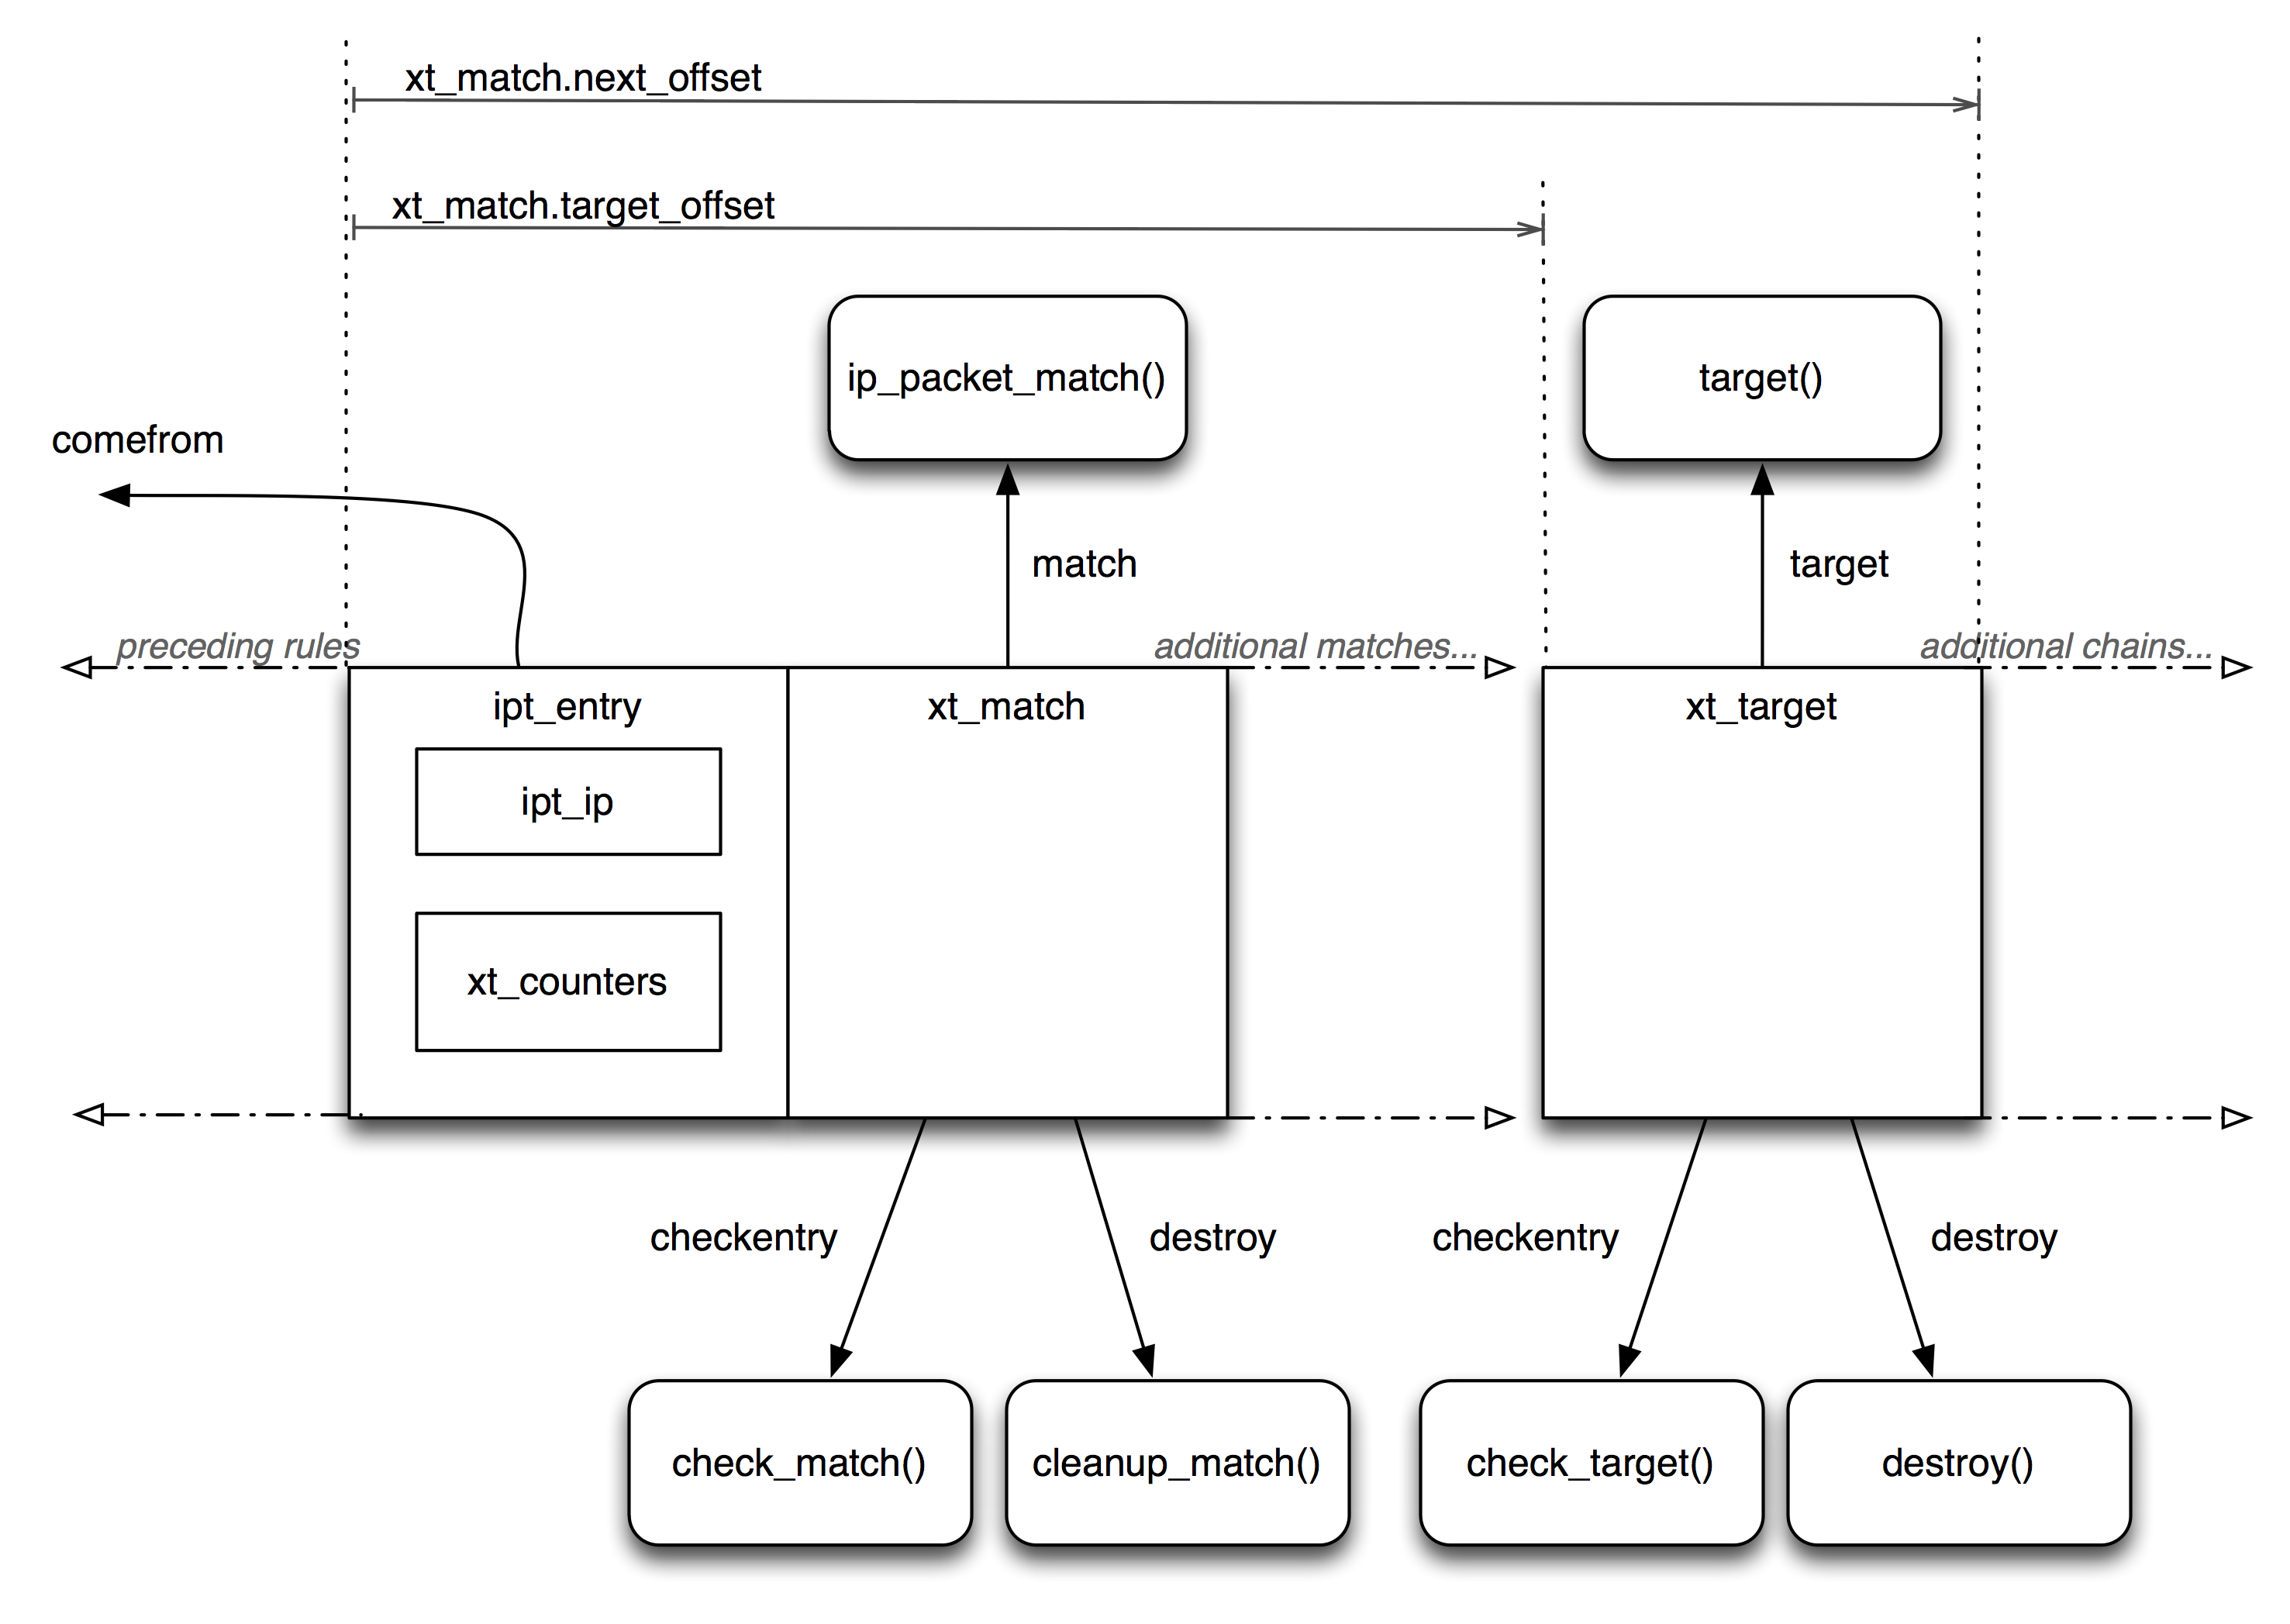
\includegraphics[totalheight=0.40\textheight]{images/table1.png}
\caption{The structure of an \code{iptables} IPv4 table.}\label{fig:table1}
\end{figure}

\subsection{Execution}

\subsubsection{ip\_tables.h/IPT\_MATCH\_ITERATE}

For historical reasons, the IP specific \code{IPT\_MATCH\_ITERATE}
macro calls the more general \code{XT\_MATCH\_ITERATE}. 

\begin{lstlisting}
  /* fn returns 0 to continue iteration */
#define IPT_MATCH_ITERATE(e, fn, args...) \
	XT_MATCH_ITERATE(struct ipt_entry, e, fn, ## args)
\end{lstlisting}

Similarly, the IPv4 specific \code{IPT\_ENTRY\_ITERATE} calls
\code{XT\_ENTRY\_ITERATE} to iterate through the rule entries beginning
at \code{ipt\_entry}.

\begin{lstlisting}
  /* fn returns 0 to continue iteration */
#define IPT_ENTRY_ITERATE(entries, size, fn, args...) \
	XT_ENTRY_ITERATE(struct ipt_entry, entries, size, fn, ## args)
\end{lstlisting}

\subsubsection{XT\_MATCH\_ITERATE}

The \code{XT\_MATCH\_ITERATE} macro expands to a for loop that
iterates through the list of \code{xt\_match} structures starting from
the \code{ipt\_entry}. With each step, the index into the rule is
advanced by the length of the current \code{xp\_match} object and the
associated match function is called. If the match functions returns 0,
i.e. the packet matches, the iteration continues.


\begin{lstlisting}
/* fn returns 0 to continue iteration */
#define XT_MATCH_ITERATE(type, e, fn, args...)			\
({								\
	unsigned int __i;					\
	int __ret = 0;						\
	struct xt_entry_match *__m;				\
								\
	for (__i = sizeof(type);				\
	     __i < (e)->target_offset;				\
	     __i += __m->u.match_size) {			\
		__m = (void *)e + __i;				\
								\
		__ret = fn(__m , ## args);			\
		if (__ret != 0)					\
			break;					\
	}							\
	__ret;							\
})

\end{lstlisting}


\subsubsection{XT\_ENTRY\_ITERATE\_CONTINUE and XT\_ENTRY\_ITERATE}

The \code{XT\_ENTRY\_ITERATE\_CONTINUE} and \code{XT\_ENTRY\_ITERATE}
macros are used whenever it is necessary to walk through a table
applying the function \code{fn} on each
entry\footnote{\code{XT\_ENTRY\_ITERATE} skips the application of
  \code{fn} on the first entry.}.

\begin{lstlisting}
/* fn returns 0 to continue iteration */
#define XT_ENTRY_ITERATE(type, entries, size, fn, args...) \
	XT_ENTRY_ITERATE_CONTINUE(type, entries, size, 0, fn, args)

/* fn returns 0 to continue iteration */
#define XT_ENTRY_ITERATE_CONTINUE(type, entries, size, n, fn, args...) \
({								\
	unsigned int __i, __n;					\
	int __ret = 0;						\
	type *__entry;						\
								\
	for (__i = 0, __n = 0; __i < (size);			\
	     __i += __entry->next_offset, __n++) { 		\
		__entry = (void *)(entries) + __i;		\
		if (__n < n)					\
			continue;				\
								\
		__ret = fn(__entry , ## args);			\
		if (__ret != 0)					\
			break;					\
	}							\
	__ret;							\
})
\end{lstlisting}


\subsubsection{ip\_tables.c/ip\_packet\_match}

Below is the basic match function that is performed on the header of
every incoming packet (with some debugging statements omitted). Lines
12-17 apply the netmask from the rule to the source and destination
IPs of the packet header \code{iphdr} and verifies that they
correspond to the fields in \code{ipt\_ip}(\ref{ipt_ip}). It also
verifies that the rule is checking source and destination
addresses. Lines 19-29 verify that the incoming and outgoing interface
of the packet correspond to the rule and that the rule checks for
interfaces. Lines 31-35 verify the protocol matches and that the
protocol is being checked. The final check on line 39 verifies that if
the match applies to fragmented packets, that the packet is
fragmented.


\lstset{stepnumber=1,frame=single,numbers=left,numberstyle=\footnotesize}

\begin{lstlisting}
static inline bool
ip_packet_match(const struct iphdr *ip,
		const char *indev,
		const char *outdev,
		const struct ipt_ip *ipinfo,
		int isfrag)
{
	unsigned long ret;

#define FWINV(bool, invflg) ((bool) ^ !!(ipinfo->invflags & (invflg)))

	if (FWINV((ip->saddr&ipinfo->smsk.s_addr) != ipinfo->src.s_addr,
		  IPT_INV_SRCIP)
	    || FWINV((ip->daddr&ipinfo->dmsk.s_addr) != ipinfo->dst.s_addr,
		     IPT_INV_DSTIP)) {
		return false;
	}

	ret = ifname_compare_aligned(indev, ipinfo->iniface, ipinfo->iniface_mask);

	if (FWINV(ret != 0, IPT_INV_VIA_IN)) {
		return false;
	}

	ret = ifname_compare_aligned(outdev, ipinfo->outiface, ipinfo->outiface_mask);

	if (FWINV(ret != 0, IPT_INV_VIA_OUT)) {
		return false;
	}

	/* Check specific protocol */
	if (ipinfo->proto
	    && FWINV(ip->protocol != ipinfo->proto, IPT_INV_PROTO)) {
		return false;
	}

	/* If we have a fragment rule but the packet is not a fragment
	 * then we return zero */
	if (FWINV((ipinfo->flags&IPT_F_FRAG) && !isfrag, IPT_INV_FRAG)) {
		return false;
	}

	return true;
}
\end{lstlisting}

\subsubsection{do\_match}
The \code{do\_match} function is the function called by the
\code{XT\_MATCH\_ITERATOR} macro. It executes the match routine
associated with each match entry in the rule, for example it would call
\code{ip\_packet\_match} above for a basic IPv4 match.

\lstset{stepnumber=0}
\begin{lstlisting}
 static inline bool
do_match(struct ipt_entry_match *m, const struct sk_buff *skb,
	 struct xt_match_param *par)
{
	par->match     = m->u.kernel.match;
	par->matchinfo = m->data;

	/* Stop iteration if it doesn't match */
	if (!m->u.kernel.match->match(skb, par))
		return true;
	else
		return false;
}
\end{lstlisting}

\subsubsection{do\_table}

\begin{lstlisting}
  /* Returns one of the generic firewall policies, like NF_ACCEPT. */
unsigned int
ipt_do_table(struct sk_buff *skb,
	     unsigned int hook,
	     const struct net_device *in,
	     const struct net_device *out,
	     struct xt_table *table)
{
#define tb_comefrom ((struct ipt_entry *)table_base)->comefrom

	static const char nulldevname[IFNAMSIZ] __attribute__((aligned(sizeof(long))));
	const struct iphdr *ip;
	u_int16_t datalen;
	bool hotdrop = false;
	/* Initializing verdict to NF_DROP keeps gcc happy. */
	unsigned int verdict = NF_DROP;
	const char *indev, *outdev;
	void *table_base;
	struct ipt_entry *e, *back;
	struct xt_table_info *private;
	struct xt_match_param mtpar;
	struct xt_target_param tgpar;

	/* Initialization */
	ip = ip_hdr(skb);
	datalen = skb->len - ip->ihl * 4;
	indev = in ? in->name : nulldevname;
	outdev = out ? out->name : nulldevname;
	/* We handle fragments by dealing with the first fragment as
	 * if it was a normal packet.  All other fragments are treated
	 * normally, except that they will NEVER match rules that ask
	 * things we don't know, ie. tcp syn flag or ports).  If the
	 * rule is also a fragment-specific rule, non-fragments won't
	 * match it. */
	mtpar.fragoff = ntohs(ip->frag_off) & IP_OFFSET;
	mtpar.thoff   = ip_hdrlen(skb);
	mtpar.hotdrop = &hotdrop;
	mtpar.in      = tgpar.in  = in;
	mtpar.out     = tgpar.out = out;
	mtpar.family  = tgpar.family = NFPROTO_IPV4;
	mtpar.hooknum = tgpar.hooknum = hook;

	IP_NF_ASSERT(table->valid_hooks & (1 << hook));
	xt_info_rdlock_bh();
	private = table->private;
	table_base = private->entries[smp_processor_id()];

	e = get_entry(table_base, private->hook_entry[hook]);

	/* For return from builtin chain */
	back = get_entry(table_base, private->underflow[hook]);

	do {
		struct ipt_entry_target *t;

		IP_NF_ASSERT(e);
		IP_NF_ASSERT(back);
		if (!ip_packet_match(ip, indev, outdev,
		    &e->ip, mtpar.fragoff) ||
		    IPT_MATCH_ITERATE(e, do_match, skb, &mtpar) != 0) {
			e = ipt_next_entry(e);
			continue;
		}

		ADD_COUNTER(e->counters, ntohs(ip->tot_len), 1);

		t = ipt_get_target(e);
		IP_NF_ASSERT(t->u.kernel.target);

#if defined(CONFIG_NETFILTER_XT_TARGET_TRACE) || \
    defined(CONFIG_NETFILTER_XT_TARGET_TRACE_MODULE)
		/* The packet is traced: log it */
		if (unlikely(skb->nf_trace))
			trace_packet(skb, hook, in, out,
				     table->name, private, e);
#endif
		/* Standard target? */
		if (!t->u.kernel.target->target) {
			int v;

			v = ((struct ipt_standard_target *)t)->verdict;
			if (v < 0) {
				/* Pop from stack? */
				if (v != IPT_RETURN) {
					verdict = (unsigned)(-v) - 1;
					break;
				}
				e = back;
				back = get_entry(table_base, back->comefrom);
				continue;
			}
			if (table_base + v != ipt_next_entry(e)
			    && !(e->ip.flags & IPT_F_GOTO)) {
				/* Save old back ptr in next entry */
				struct ipt_entry *next = ipt_next_entry(e);
				next->comefrom = (void *)back - table_base;
				/* set back pointer to next entry */
				back = next;
			}

			e = get_entry(table_base, v);
			continue;
		}

		/* Targets which reenter must return
		   abs. verdicts */
		tgpar.target   = t->u.kernel.target;
		tgpar.targinfo = t->data;


#ifdef CONFIG_NETFILTER_DEBUG
		tb_comefrom = 0xeeeeeeec;
#endif
		verdict = t->u.kernel.target->target(skb, &tgpar);
#ifdef CONFIG_NETFILTER_DEBUG
		if (tb_comefrom != 0xeeeeeeec && verdict == IPT_CONTINUE) {
			printk("Target %s reentered!\n",
			       t->u.kernel.target->name);
			verdict = NF_DROP;
		}
		tb_comefrom = 0x57acc001;
#endif
		/* Target might have changed stuff. */
		ip = ip_hdr(skb);
		datalen = skb->len - ip->ihl * 4;

		if (verdict == IPT_CONTINUE)
			e = ipt_next_entry(e);
		else
			/* Verdict */
			break;
	} while (!hotdrop);
	xt_info_rdunlock_bh();

#ifdef DEBUG_ALLOW_ALL
	return NF_ACCEPT;
#else
	if (hotdrop)
		return NF_DROP;
	else return verdict;
#endif

#undef tb_comefrom
}
\end{lstlisting}

\section{ConnTrack}\label{conntrack}

\subsection{Overview}
The \verb|conntrack| system provides connection tracking so that as each packet is processed, its context within in a connection is known. This allows for more intelligent filtering decisions to be made and is essential to implement a so-called \textit{stateful firewall}, as opposed to a simple packet filter. Other modules that require connection tracking are built on top of the basic functionality provided by \verb|conntrack|.

\subsection{Data Structures}

\subsubsection{nf\_conntrack\_tuple.h/nf\_conntrack\_tuple}\label{nf_conntrack_tuple}

The \code{nf\_conntrack\_tuple} structure is used to uniquely identify
a connection that has passed through the firewall and whose state is
being tracked. The \code{src} field is the source address, which is
considered manipulable (useful for NAT), unlike the remaining fields,
which are immutable. The field \code{u3} represents the destination
address in either IPv4 and IPv6, depending on what type of packet is
being tracked. The union \code{u} with \code{tcp}, \code{udp},
\code{icmp}, etc., track layer 4 protocol state fields for the
destination, such as the port number for TCP\cite{tcpip-illustrated}. The \code{all} field is
used when multiple fields need to be accessed at once, e.g. for
hashing of the tuple. Finally, \code{protonum} stores the protocol in
use, (TCP or UDP, etc.) and \code{dir} stores the direction.

\begin{lstlisting}
struct nf_conntrack_tuple
{
	struct nf_conntrack_man src;

	struct {
		union nf_inet_addr u3;
		union {
			/* Add other protocols here. */
			__be16 all;

			struct {
				__be16 port;
			} tcp;
			struct {
				__be16 port;
			} udp;
			struct {
				u_int8_t type, code;
			} icmp;
			struct {
				__be16 port;
			} dccp;
			struct {
				__be16 port;
			} sctp;
			struct {
				__be16 key;
			} gre;
		} u;

		/* The protocol. */
		u_int8_t protonum;

		/* The direction (for tuplehash) */
		u_int8_t dir;
	} dst;
};
\end{lstlisting}

\subsubsection{nf\_conntrack\_tuple.h/nf\_conntrack\_tuple\_hash}\label{nf_conntrack_tuple_hash}

\begin{lstlisting}
  /* Connections have two entries in the hash table: one for each way */
struct nf_conntrack_tuple_hash {
	struct hlist_nulls_node hnnode;
	struct nf_conntrack_tuple tuple;
};
\end{lstlisting}

\subsubsection{nf\_conntrack\_tuple.h/ip\_conntrack\_old\_tuple}

This is an old IPv4 specific format for the tuple. It is kept for
historical reasons since it has been exposed to userspace.

\begin{lstlisting}
/* This is exposed to userspace, so remains frozen in time. */
struct ip_conntrack_old_tuple
{
	struct {
		__be32 ip;
		union {
			__u16 all;
		} u;
	} src;

	struct {
		__be32 ip;
		union {
			__u16 all;
		} u;

		/* The protocol. */
		__u16 protonum;
	} dst;
};
\end{lstlisting}

\subsubsection{nf\_conntrack\_tuple.h/xt\_conntrack\_info}

\begin{lstlisting}
struct xt_conntrack_info
{
	unsigned int statemask, statusmask;

	struct ip_conntrack_old_tuple tuple[IP_CT_DIR_MAX];
	struct in_addr sipmsk[IP_CT_DIR_MAX], dipmsk[IP_CT_DIR_MAX];

	unsigned long expires_min, expires_max;

	/* Flags word */
	__u8 flags;
	/* Inverse flags */
	__u8 invflags;
};
\end{lstlisting}



\subsubsection{nf\_conntrack.h/nf\_conn}\label{nf_conn}

The \code{ct\_general} is an atomic counter that tracks the usage of
the \code{nf\_conn} structure. The spinlock is used to protect the
connection on SMP systems. The \verb|tuplehash| is a two element array
that contains the tuple for the initiating side of the connection
(index \verb|IP_CT_DIR_ORIGINAL|) and a second tuple for the
reply packet (index \verb|IP_CT_DIR_ORIGINAL|). The reply tuple
can be easily calculated by inverting fields. For example in a TCP
connection, to generate the reply tuple, the source and destination IP
addresses of the initial packet are inverted, as are the source and
destination port numbers.

\begin{lstlisting}
  struct nf_conn {
	/* Usage count in here is 1 for hash table/destruct timer, 1 per skb,
           plus 1 for any connection(s) we are `master' for */
	struct nf_conntrack ct_general;

	spinlock_t lock;

	/* These are my tuples; original and reply */
	struct nf_conntrack_tuple_hash tuplehash[IP_CT_DIR_MAX];

	/* Have we seen traffic both ways yet? (bitset) */
	unsigned long status;

	/* If we were expected by an expectation, this will be it */
	struct nf_conn *master;

	/* Timer function; drops refcnt when it goes off. */
	struct timer_list timeout;

#if defined(CONFIG_NF_CONNTRACK_MARK)
	u_int32_t mark;
#endif

#ifdef CONFIG_NF_CONNTRACK_SECMARK
	u_int32_t secmark;
#endif

	/* Storage reserved for other modules: */
	union nf_conntrack_proto proto;

	/* Extensions */
	struct nf_ct_ext *ext;
#ifdef CONFIG_NET_NS
	struct net *ct_net;
#endif
};
\end{lstlisting}

\subsubsection{conntrack.h/netns\_ct}

This points to global connection tracking entities like the
\verb|expect_hash| hash table for expected packets. The atomic
\verb|count| refers to the number of active connections being tracked
through the firewall, and \verb|hash| points to the hash table for
active connections. The \verb|unconfirmed| table is where tuples are
temporarily stashed before the corresponding packet leaves the
firewall.

\begin{lstlisting}
  struct netns_ct {
	atomic_t		count;
	unsigned int		expect_count;
	struct hlist_nulls_head	*hash;
	struct hlist_head	*expect_hash;
	struct hlist_nulls_head	unconfirmed;
	struct hlist_nulls_head	dying;
	struct ip_conntrack_stat *stat;
	int			sysctl_events;
	unsigned int		sysctl_events_retry_timeout;
	int			sysctl_acct;
	int			sysctl_checksum;
	unsigned int		sysctl_log_invalid; /* Log invalid packets */
#ifdef CONFIG_SYSCTL
	struct ctl_table_header	*sysctl_header;
	struct ctl_table_header	*acct_sysctl_header;
	struct ctl_table_header	*event_sysctl_header;
#endif
	int			hash_vmalloc;
	int			expect_vmalloc;
};
\end{lstlisting}

\subsubsection{nf\_conntrack\_expect.h/nf\_conntrack\_expect}

\begin{lstlisting}
  struct nf_conntrack_expect
{
	/* Conntrack expectation list member */
	struct hlist_node lnode;

	/* Hash member */
	struct hlist_node hnode;

	/* We expect this tuple, with the following mask */
	struct nf_conntrack_tuple tuple;
	struct nf_conntrack_tuple_mask mask;

	/* Function to call after setup and insertion */
	void (*expectfn)(struct nf_conn *new,
			 struct nf_conntrack_expect *this);

	/* Helper to assign to new connection */
	struct nf_conntrack_helper *helper;

	/* The conntrack of the master connection */
	struct nf_conn *master;

	/* Timer function; deletes the expectation. */
	struct timer_list timeout;

	/* Usage count. */
	atomic_t use;

	/* Flags */
	unsigned int flags;

	/* Expectation class */
	unsigned int class;

#ifdef CONFIG_NF_NAT_NEEDED
	__be32 saved_ip;
	/* This is the original per-proto part, used to map the
	 * expected connection the way the recipient expects. */
	union nf_conntrack_man_proto saved_proto;
	/* Direction relative to the master connection. */
	enum ip_conntrack_dir dir;
#endif

	struct rcu_head rcu;
};
\end{lstlisting}


\subsubsection{Diagram}

The hash table shown in diagram \figref{fig:hash} is used to store
tuples for established connections. Each entry points to a list of tuples
with the same hash key. New tuples are inserted at the head.

The efficiency of this structure is extremely important since a packet's tuple must be
looked up every time it arrives on an interface or is sent from an
internal process. Space must also be considered because the table can
grow quite large on a busy firewall handling thousands of connections
concurrently.

One space optimization was the use of
\verb|hlist_node| and \verb|hlist_head| over the more general \verb|list_head|. The
latter has a pointer to the tail of the list, which means the tail can
be reached in $O(N)$ time. However, since this is not needed for tuple
look-ups\footnote{Tuple collisions are inserted in front -- there is
  no reason to jump to the tail.}, the extra pointer in
\verb|list_head| is superfluous. The \verb|hlist_head| contains only a
\verb|first| pointer field. Although, this creates another
complication: when accessing the previous node (e.g. for insertion) it
is no longer known whether it is a \verb|hlist_node.next| or a
\verb|hlist_head.first|. To get around this, the \verb|pprev| field is
a pointer to a pointer -- a pointer to whatever field is pointing to
the current node. Thus, for insertions and deletions, the previous node/head can be
updated regardless of type.

To access the containing structure of an \verb|hlist_node|, in this
case an \verb|nf_conntrack_tuple_hash|, the macro
\verb|container_of| is used to cleverly calculate
the address containing structure address from the member address.

\begin{lstlisting}
  #define container_of(ptr, type, member) ({			\
	const typeof( ((type *)0)->member ) *__mptr = (ptr);	\
	(type *)( (char *)__mptr - offsetof(type,member) );})
\end{lstlisting}


\begin{sidewaysfigure}
  \centering
  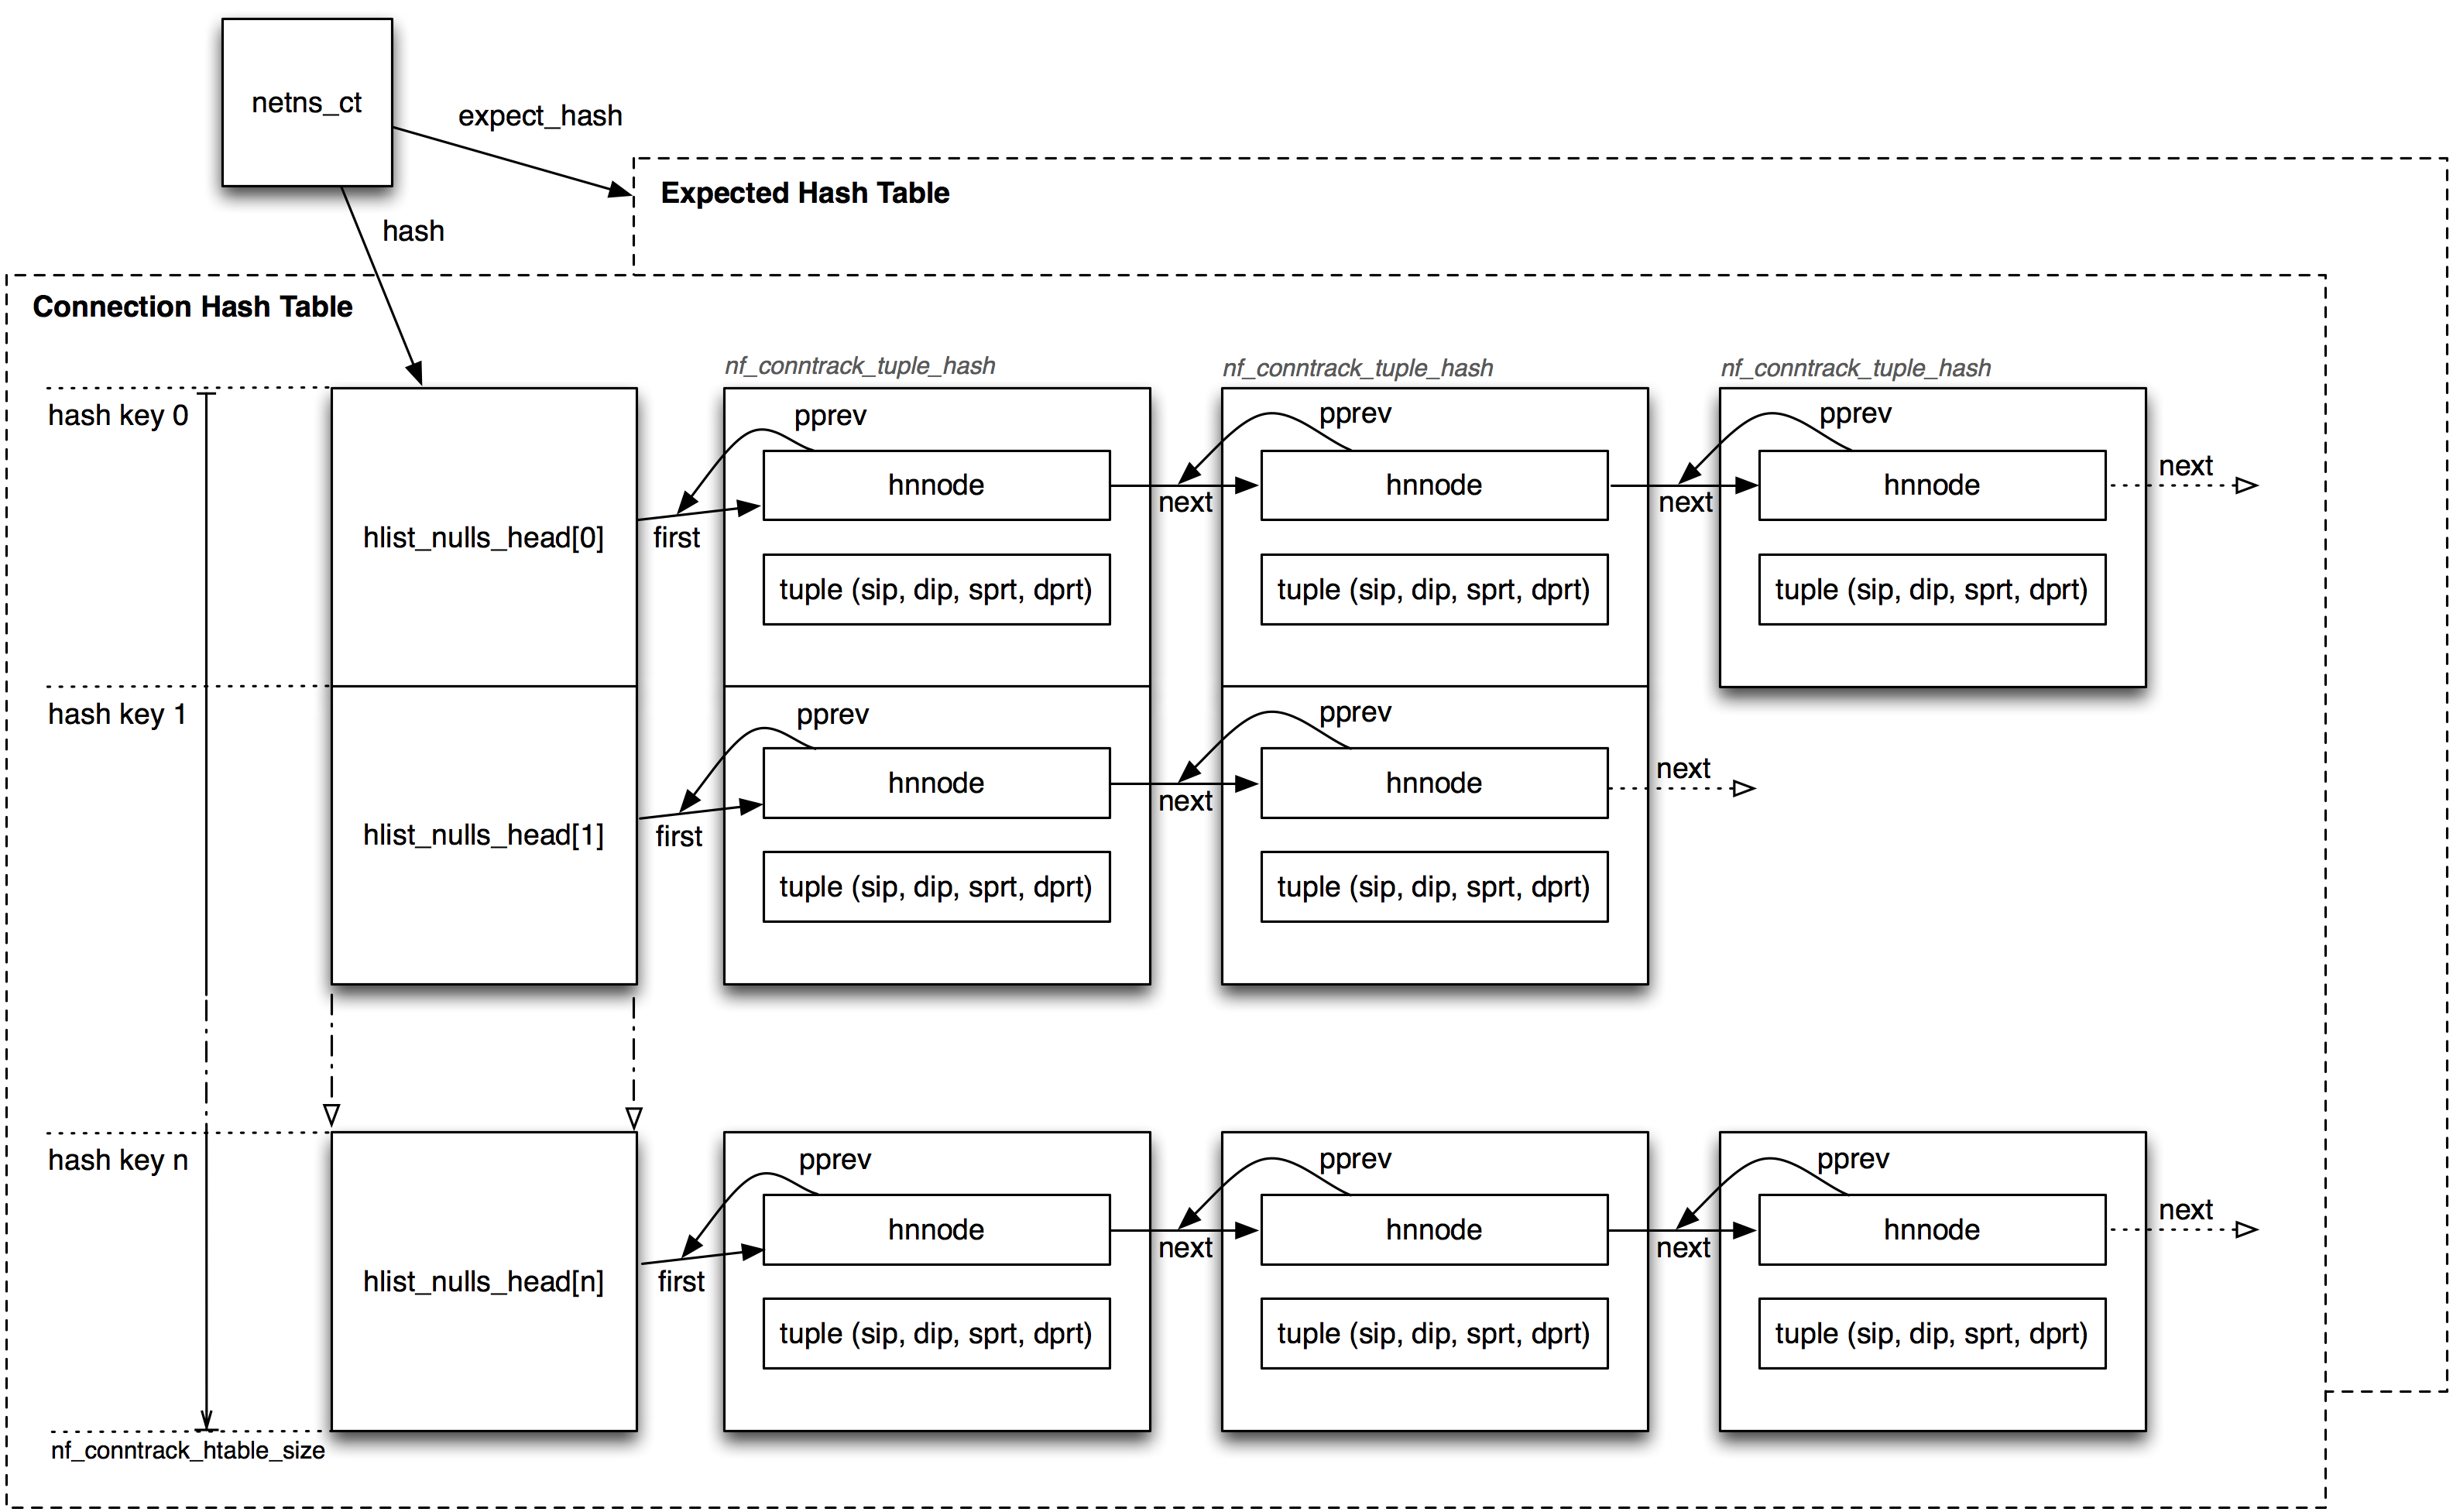
\includegraphics[totalheight=0.60\textheight]{images/hash_expect_tables.png}
  \caption{The structure of the hash tables that store active
    connections (\code{hash} pointer) and expected connections
    (\code{expect\_hash}).}\label{fig:hash}
\end{sidewaysfigure}

\subsection{Execution}

\begin{figure}[H]
  \centering
  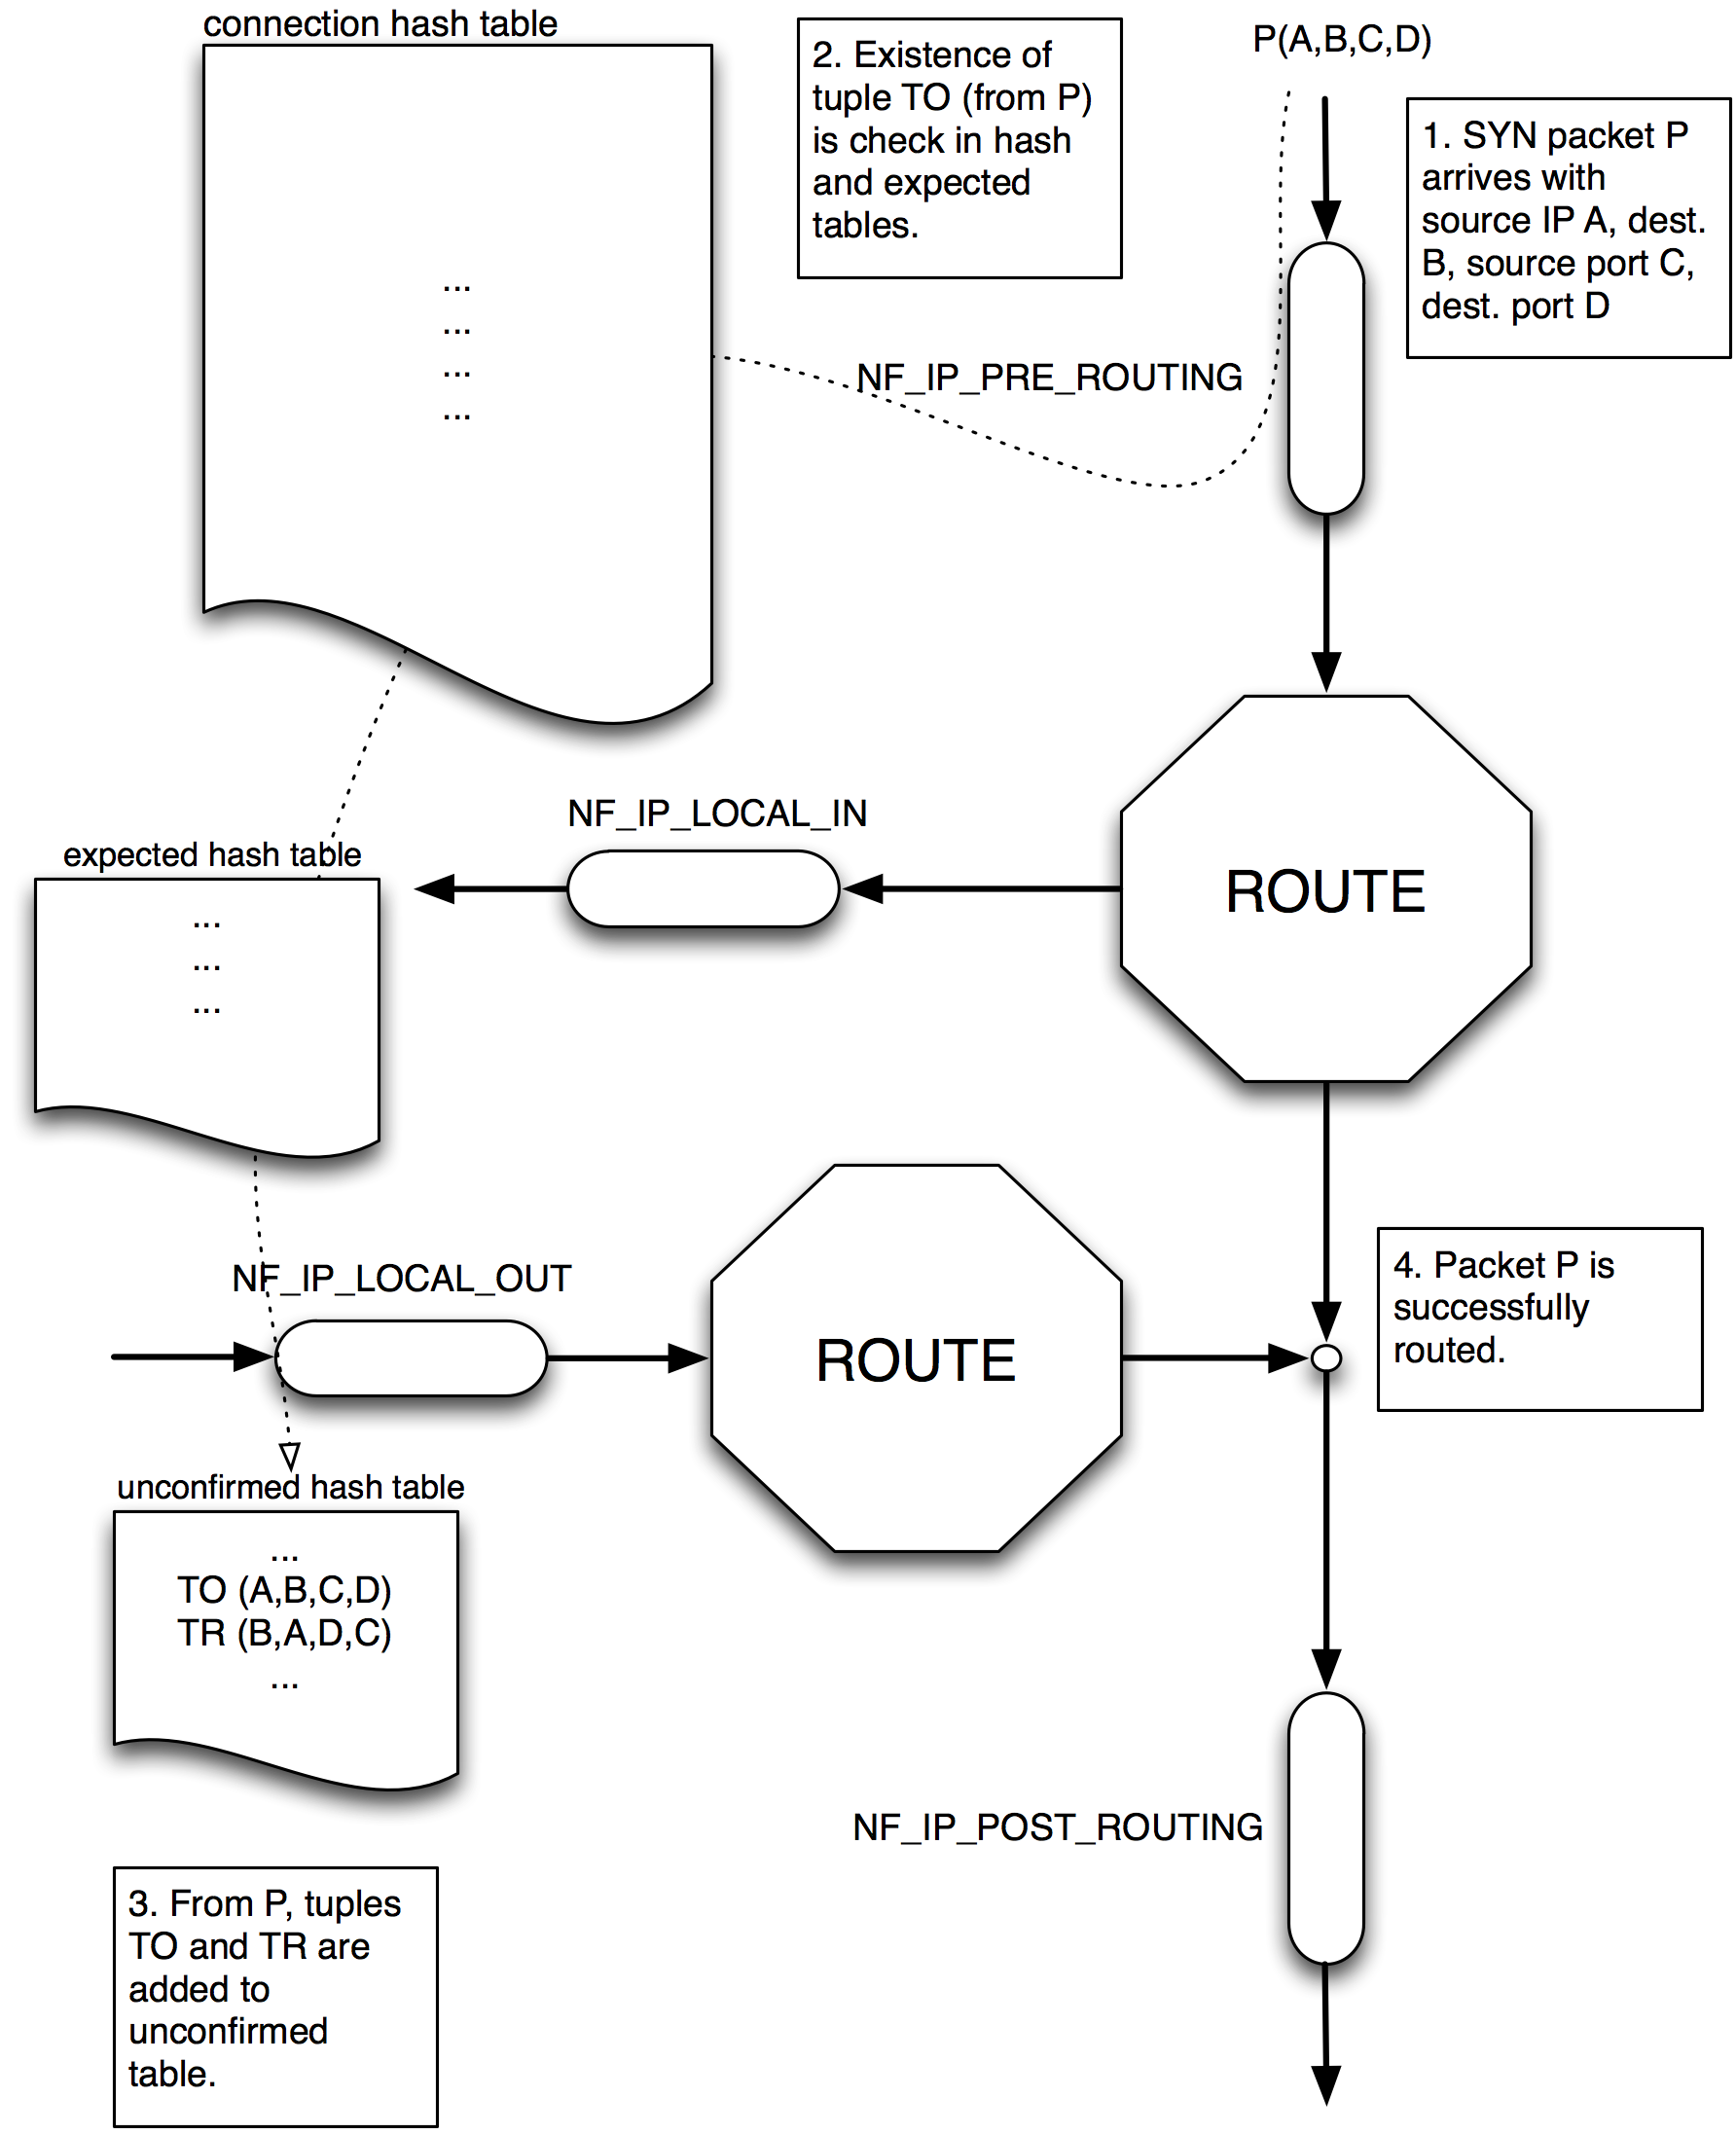
\includegraphics[totalheight=0.90\textheight]{images/conntrack_flow1.png}
  \caption{Part 1. New connection packet P enters the firewall.}\label{fig:conntrack_flow1}
\end{figure}

\begin{figure}[H]
  \centering
  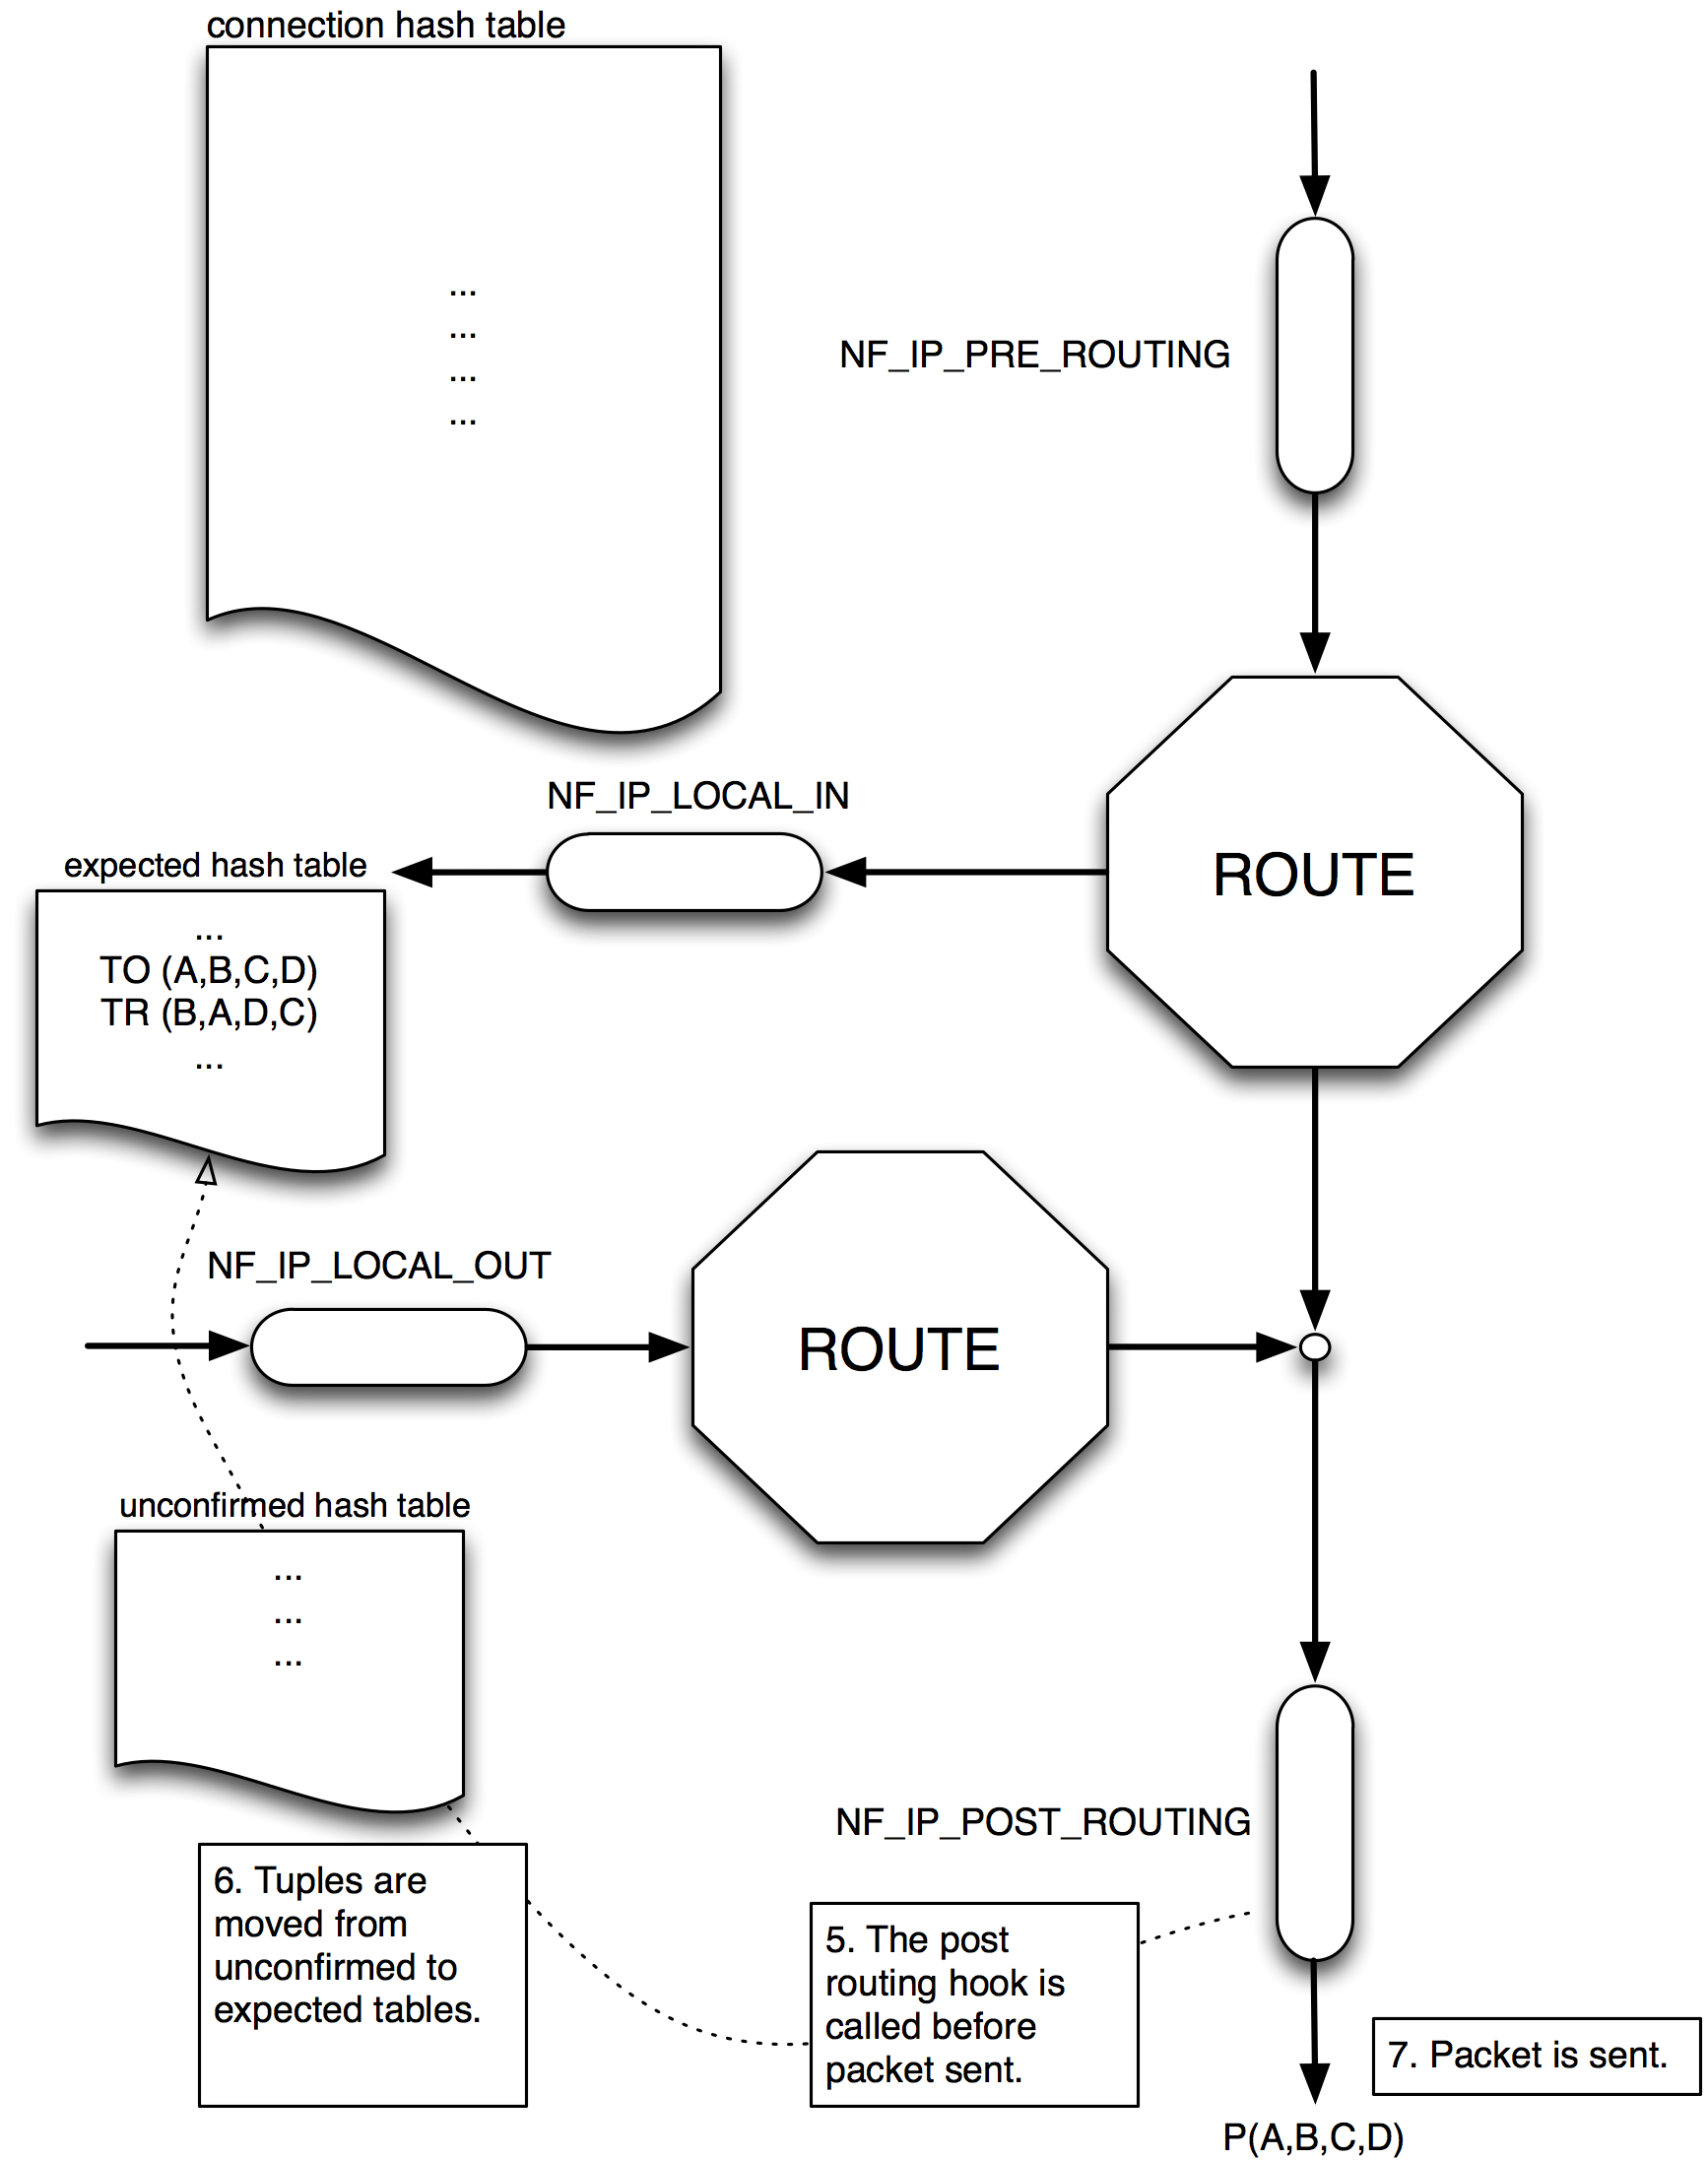
\includegraphics[totalheight=0.90\textheight]{images/conntrack_flow2.png}
  \caption{Part 2. Packet P is confirmed and leaves the firewall.}\label{fig:conntrack_flow2}
\end{figure}

\begin{figure}[H]
  \centering
  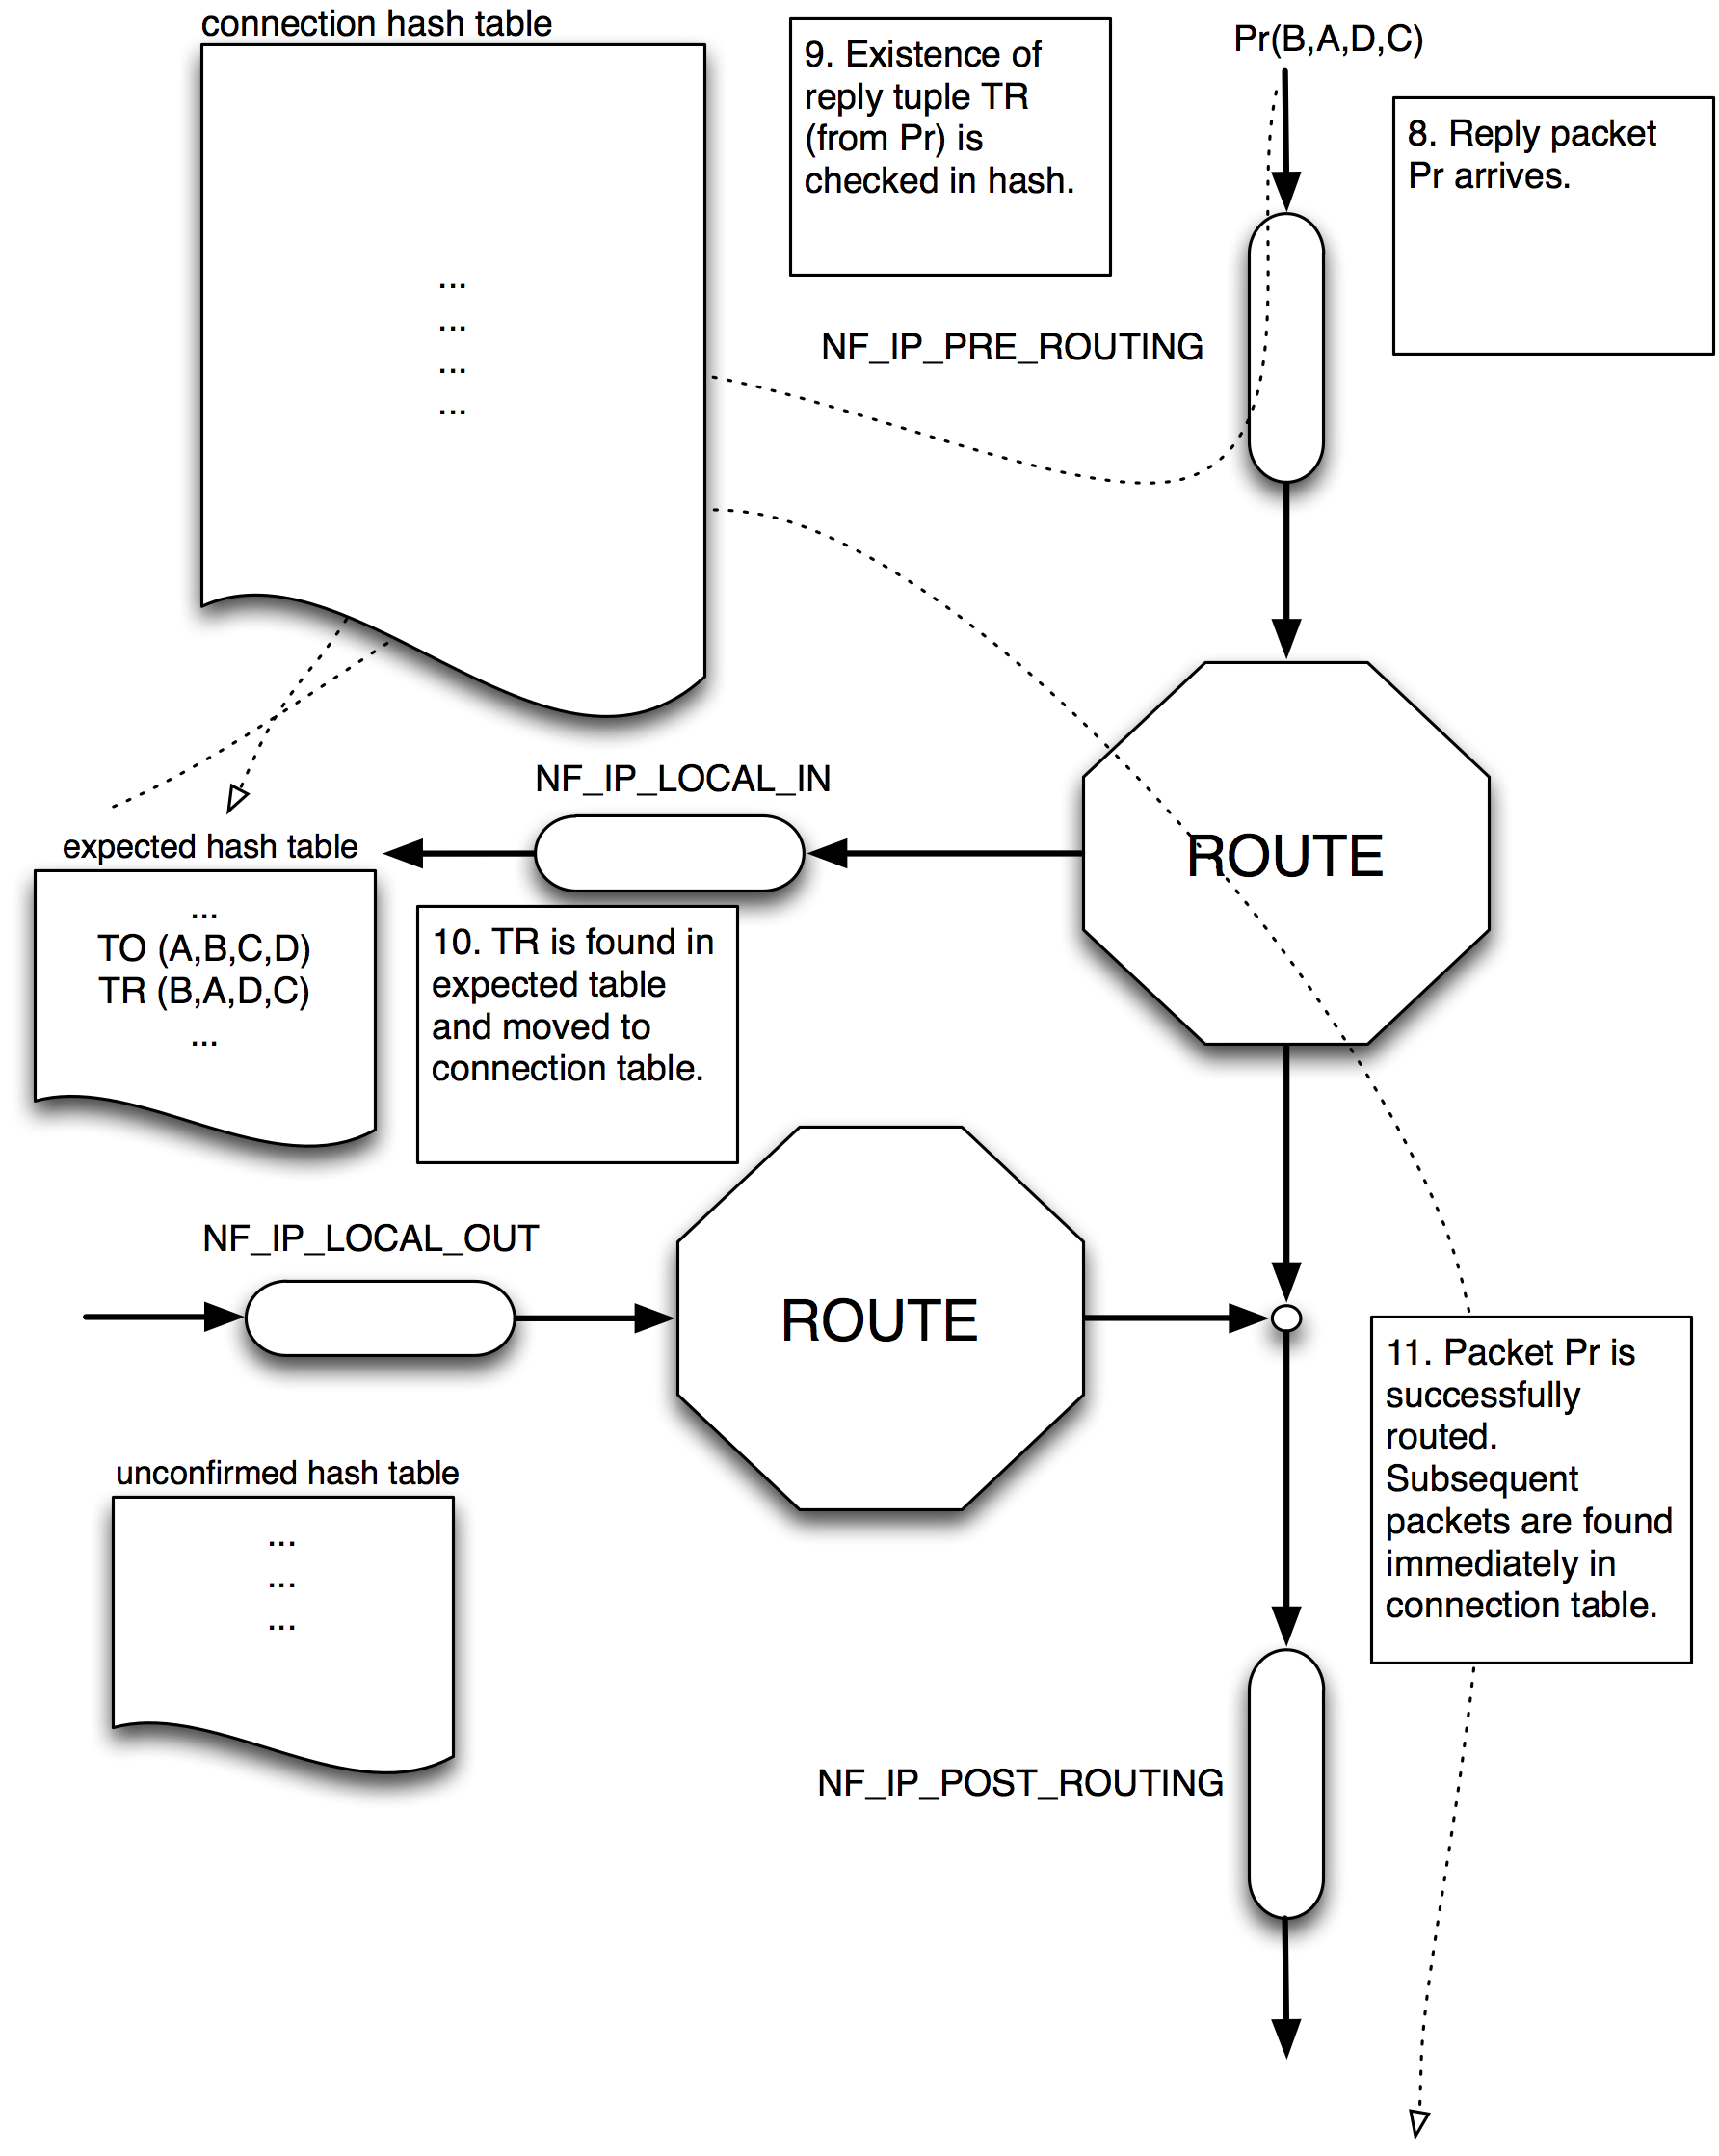
\includegraphics[totalheight=0.90\textheight]{images/conntrack_flow3.png}
  \caption{Part 3. Reply packet Pr returns and the connection is established.}\label{fig:conntrack_flow3}
\end{figure}

\subsubsection{Initiating a new connection}

When a packet arrives on an interface or is sent by a local process,
it triggers the \verb|PRE_ROUTING| or \verb|LOCAL_OUT| hooks
respectively\figref{fig:hooks}. The \verb|conntrack| module is always called first
because it is registered with the highest priority. The packet's tuple
is calculated\cite{jhash} and looked-up in the \verb|hash| \figref{fig:hash} table
for existing connections and \verb|expect_hash| for expected
connections (explained in \ref{reply}). If the packet is the
initiating packet of a new connection (e.g. a SYN packet for a TCP
connection\cite{tcpip-illustrated}) it will not be found. Instead, its tuple (in
\verb|nf_conntrack_tuple_hash| \cref{nf_conntrack_tuple_hash}) and
reverse tuple(\ref{nf_conn}) are added to the \verb|unconfirmed| table
in the \verb|netns_ns| structure. The packet is then passed on for
routing. However, there is some chance that the packet may not emerge,
for instance, if there is no valid route or it is dropped by a
subsequent rule\cite{netfilter-internals}. In this scenario, the
tuples will eventually time-out and be culled from \verb|unconfirmed|.
On the other hand, if it is routed successfully the
\verb|POST_ROUTING| hook is called. The initiating tuple the reverse
tuple is transferred from \verb|unconfirmed| to \verb|hash_expect|. At
this point it can be assumed the packet will leave the host.

\subsubsection{Reply to new connection}\label{reply}
When the reply packet returns to the firewall, it again triggers the
\verb|PRE_ROUTING| hook. This time the reply tuple is found in
\verb|expect_hash| and then transferred to \verb|hash| for established
connections. Any subsequent packets related to this connection will
found immediately in the \verb|hash| table. The state of any given
packet is made available to the rest of the kernel through the socket buffer struct
\verb|sk_buff.nfct|.

\section{Registration}\label{registration}



% hook registration section

\subsection{Hook Object}\label{hook_object}
To be able to register a hook, the \verb|nf_register_hook|takes a struct of type \verb|nf_hook_ops, which is a structure hook to be added to the list of hooks and its options.
From Victor Castro's description: ``The first thing we see in the struct is the list_head struct, which is used to keep a linked list of hooks, but it's not necessary for our firewall. The \verb{nf_hookfn*} struct member is the name of the hook function that we define. The pf integer member is used to identify the protocol family; it's \verb{PF_INET} for IPv4. The next field is the hooknum int, and this is for the hook we want to use. The last field is the priority int. The priorities are specified in \verb|linux/netfilter_ipv4.h|, but for our situation we want \verb{NF_IP_PRI_FIRST}.''\cite{netfilter-firewall}
The list_head struct inside of the nf_hook_ops will be covered in more detail in section \ref{hook_add} and why it's needed.
\cite{netfilter-firewall}

\begin{lstlisting}
struct nf_hook_ops
{
	struct list_head list;

	/* User fills in from here down. */
	nf_hookfn	*hook;
	struct module	*owner;
	void		*priv;
	u_int8_t	pf;
	unsigned int	hooknum;
	/* Hooks are ordered in ascending priority. */
	int		priority;
};
\end{lstlisting}

\subsection{Hook List Object}\label{hook_list_object}
The hook list object is a standard double linked list object used throughout the kernel. It's definition \verb|list_head| and utility functions are defined in \verb|include/linux/list.h| and allows for standard linked list functionality. A linked list is a perfect data structure in this case since there is no specific element indexing, but rather traversing through the list and calling all the available hooks. There are 6 hooks lists. One for each of \verb|NF_INET_PRE_ROUTING| , \verb|NF_INET_LOCAL_IN|, \verb|NF_INET_FORWARD|, \verb|NF_INET_LOCAL_OUT|, \verb|NF_INET_POST_ROUTING|. By breaking the lists into one for each hook spot, on every spot where the hooks need to be called only the hooks responsible for that spot are iterated.

\begin{lstlisting}
extern struct list_head nf_hooks[NFPROTO_NUMPROTO][NF_MAX_HOOKS];
\end{lstlisting}

\subsection{Hook Adding}\label{hook_add}
The kernel attempts to add the hook object passed, by first creating a nf_hook_mutex object, locking it until it has finnished the hook adding process. It then adds the given hook object by using the \verb|struct list_head list| as the reference pointer inside of the linked list but before adding it, loops through the list so that the list remains sorted by priority. That way when the hooks are called there is no need for sorting and the hooks with higher priority are called first. It unlocks the mutex and finally it adds the \verb|nf_register_hook| function to the modules API. This allows the function to be used from loaded modules. 

\begin{lstlisting}
int nf_register_hook(struct nf_hook_ops *reg)
{
	struct nf_hook_ops *elem;
	int err;

	err = mutex_lock_interruptible(&nf_hook_mutex);
	if (err < 0)
		return err;
	list_for_each_entry(elem, &nf_hooks[reg->pf][reg->hooknum], list) {
		if (reg->priority < elem->priority)
			break;
	}
	list_add_rcu(&reg->list, elem->list.prev);
	mutex_unlock(&nf_hook_mutex);
	return 0;
}
EXPORT_SYMBOL(nf_register_hook);
\end{lstlisting}

\subsection{Hook List Adding}\label{hook_list_adding}
The functionality to add several hooks at once also is available by letting the user provide an array of \verb|nf_hook_ops| and loop-add them to the linked list.

\begin{lstlisting}
int nf_register_hooks(struct nf_hook_ops *reg, unsigned int n)
{
	unsigned int i;
	int err = 0;

	for (i = 0; i < n; i++) {
		err = nf_register_hook(&reg[i]);
		if (err)
			goto err;
	}
	return err;

err:
	if (i > 0)
		nf_unregister_hooks(reg, i);
	return err;
}
\end{lstlisting}

\subsection{Hook And Hook-List Removing}\label{hook_removing}
The hooks can also be removed from the linked list in similar fashion to the way they are added.

\begin{lstlisting}
void nf_unregister_hook(struct nf_hook_ops *reg);
void nf_unregister_hooks(struct nf_hook_ops *reg);
\end{lstlisting}

\subsection{Hooks Processing}\label{hooks_processing}
Finally there exist facilities inside \verb|netfilter.h| that allow the kernel to process the hooks that are registered at the various steps. Many are in the form of macros that add certain small functionality before the function \verb|nf_hook_slow| is called. This function iterates through all the hooks registered for the current step, executes them and proceeds according to the result returned by the hook.

\begin{lstlisting}
int nf_hook_slow(u_int8_t pf, unsigned int hook, struct sk_buff *skb,
		 struct net_device *indev, struct net_device *outdev,
		 int (*okfn)(struct sk_buff *), int thresh);
\end{lstlisting}




\bibliography{research}

\end{document}